\documentclass{article}
\usepackage{graphicx}

\begin{document}

\title{REPORT ON \\
MATRIX FACTORIZATION IN CROSS-DOMAIN RECOMMENDATIONS FRAMEWORK \\
BY SHARED USERS LATENT FACTOR}
\author{Abhishek}
\date{\today}

\maketitle
\section{Abstract}
Matrix factorization is a widely used method in collaborative filtering for personalized recommendations. However, collaborative filtering faces challenges, such as the sparsity problem, where the observed ratings are limited. To address this issue, cross-domain recommendations have been introduced, utilizing transfer learning mechanisms to enhance performance by leveraging related source domains. In this paper, the authors propose a method for knowledge transfer from a source domain to a target domain through shared users' latent factors. Traditional matrix factorization is applied in the source domain to learn latent factors of users and items. These latent factors of users are then directly transferred to the target domain, modifying the objective function of matrix factorization to learn users/items latent factors in the target domain. Experimental results demonstrate the proposed method's effectiveness in terms of Mean Absolute Error (MAE) and Root Mean Square Error (RMSE) metrics.


\section{Introduction}
Recommender systems play a crucial role in e-commerce applications, providing users with personalized recommendations from a vast pool of items. Collaborative filtering, particularly matrix factorization, has shown promise in generating these recommendations. However, the sparsity problem, where ratings are limited, poses a challenge. Cross-domain recommendations aim to mitigate this challenge by applying transfer learning from related source domains to improve the target domain's performance.

\section{Methodology}
The proposed method involves these main steps:
\begin{enumerate}
  \item The proposed method focuses on transferring knowledge from the source domain to the target domain through shared users' latent factors.
  \item Traditional matrix factorization is applied in the source domain to learn latent factors of users and items.
  \item The learned latent factors of users are directly transferred to the target domain.
  \item The objective function of matrix factorization is modified for the target domain to learn users' and items' latent factors.
  \item Predictions on unobserved ratings in the target domain are made using the inner product of the respective user and item latent factors.
\end{enumerate}

\section{Proposed Methods}

Here is an illustration of our proposed method:

\begin{figure}[h]
  \centering
  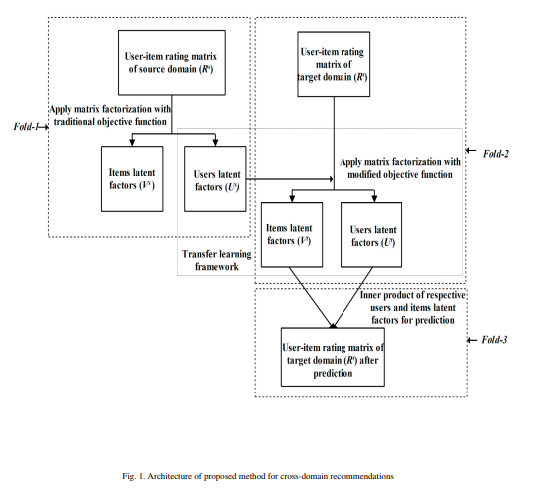
\includegraphics[width=0.8\textwidth]{mf.PNG}
  \caption{Fig. 1. Architecture of proposed method for cross-domain recommendations.}
  \label{fig:proposed_method}
\end{figure}

\section{Related Works}
The authors delve into the existing body of work related to cross-domain recommendations, with a specific emphasis on approaches categorized by the overlap of users and items between domains. Understanding the landscape of related methodologies is crucial for contextualizing the proposed method.

\subsection{Categorization of Cross-Domain Recommendation Methods}
The paper categorizes existing cross-domain recommendation methods based on the overlap of users and items between domains. This categorization helps in identifying the most relevant approaches and provides insights into the challenges and opportunities associated with each category.

\subsection{User Overlap}
In the category where users are shared between domains, the authors discuss the pioneering work by Winoto and Tang \cite{winoto_tang}, who analyzed correlations based on item categories to provide cross-domain recommendations. Subsequent research by Berkovsky et al. \cite{berkovsky} explored the import of user profile data from other domains, highlighting its positive impact on prediction accuracy. Another notable contribution in this category is the work by Pan and Yang \cite{pan_yang}, which treated like/dislike information as the source domain for transfer learning.

\subsection{Items Overlap, Users and Items Overlap}
The paper acknowledges the challenges associated with finding shared items between domains, leading to limited work in these categories. The difficulty in identifying shared items between domains poses a significant hurdle in implementing effective cross-domain recommendation systems.

\subsection{Neither Users nor Items Overlap}
The authors discuss Li et al.'s \cite{li} work, which proposed a method based on cluster-level rating patterns for knowledge transfer between domains. This method has been extended by incorporating probabilistic models \cite{probabilistic_models}. Both approaches rely on cluster-level rating patterns to establish connections between domains where neither users nor items overlap.

\subsection{Proposed Methodology}
The proposed method in this paper falls under the category of user overlap. The authors advocate for exploiting knowledge from the source domain to enhance the accuracy of the target domain by leveraging shared latent factors of users. Understanding the strengths and limitations of existing cross-domain recommendation methods informs the design and evaluation of the proposed approach. The emphasis on user overlap as a primary category showcases a strategic choice made by the authors based on the feasibility and effectiveness of knowledge transfer mechanisms.

\section{Experimental Setup}

\subsection{Dataset Preprocessing}

The experiments conducted in this study utilize the Amazon product co-purchasing network metadata \cite{amazon-meta}. The dataset involves two groups, namely 'Book' and 'DVD,' with one designated as the source domain and the other as the target. The focus is on shared users between domains, prompting the following preprocessing steps:

\begin{itemize}
    \item Filtering out items with at least 10 ratings and users who have rated at least 50 items in both domains.
    \item Matching common users using userIDs in both domains, resulting in the selection of 395 users randomly.
    \item Designating the 'Book' group as the source domain and the 'DVD' group as the target domain. It is noted that the density level of the source domain ($D_s$) is higher compared to the target domain ($D_t$).
\end{itemize}

The statistics of the filtered dataset are summarized in Table~\ref{tab:dataset-stats}.

\begin{table}[ht]
    \centering
    \caption{Statistics of Filtered Dataset}
    \label{tab:dataset-stats}
    \begin{tabular}{|c|c|c|c|c|}
        \hline
        Domain & Items with $\geq$ 10 Ratings & Users with $\geq$ 50 Ratings & Common Users \\
        \hline
        Source (Book) & $x_1$ & $y_1$ & $z_1$ \\
        Target (DVD) & $x_2$ & $y_2$ & $z_2$ \\
        \hline
    \end{tabular}
\end{table}

\subsection{Experiment Protocols}

The experimental design incorporates a 5-fold cross-validation process, ensuring unbiased results. This involves dividing the dataset into 4 parts for training and using the 5th part for testing the target domain. The overall evaluation is based on the average value across all 5 test sets. A 95\% confidence interval is employed in calculating this average. Additionally, to validate cross-domain recommendations, the training set (TR) is divided into three subparts: TR(50\%), TR(75\%), and TR(100\%).

\subsection{Evaluation Metrics}

The performance of the proposed method and other state-of-the-art techniques is assessed using Mean Absolute Error (MAE) and Root Mean Square Error (RMSE) as evaluation metrics:


Where:
\begin{itemize}
    \item $r_T$ denotes the total number of predicted ratings in the target domain.
    \item $r_{i, j}$ represents the actual rating, and $\hat{r}_{i, j}$ is the predicted rating on item $i$ for user $j$.
\end{itemize}

\subsection{Comparison Methods and Parameter Settings}

Three comparison methods are employed, along with the proposed method:

\begin{enumerate}
    \item \textbf{Average Filling (AF):}
    Predicts ratings by filling the average value of observed items' ratings given by users in the target domain.
    
    \[
    \hat{r}_{i, *} = \frac{\sum_{j=1}^{M} I_{i, j} r_{i, j}}{\sum_{j=1}^{M} I_{i, j}}
    \]

    \item \textbf{Collaborative Filtering with User-User Similarity (CF-UU):}
    Memory-based method using top $K$-NN similar users. Utilizes constrained Pearson correlation similarity formula with $K = 50$ for top $k$ users.

    \item \textbf{Matrix Factorization (MF):}
    Provides lower rank approximations of the user-item matrix. Prediction involves latent factors on the user and item sides. Parameters include $\lambda = 0.001$ (trade-off parameter), $f = 10$ (size of latent factors), and $\alpha = 0.001$.

    \item \textbf{Proposed Method:}
    Adopts adaptive transfer learning \cite{transfer-learning} \cite{adaptive-transfer-learning}, transferring knowledge from the source domain to the target domain. Parameter values are $\lambda = 0.005$, $\alpha = 0.001$, $c = 0.01$, and $f = 10$.
\end{enumerate}

The proposed method aims to enhance the accuracy of cross-domain recommendations through adaptive transfer learning.


\subsection{Advantages of the Proposed Method}
\begin{enumerate}
  \item \textbf{Adaptability:}
    \begin{itemize}
      \item The authors underscore the adaptability of their method in effectively addressing the sparsity problem within collaborative filtering.
      \item The incorporation of a transfer learning mechanism, specifically the sharing of latent factors between source and target domains, significantly enhances the model's adaptability.
    \end{itemize}
  
  \item \textbf{Robustness:}
    \begin{itemize}
      \item The proposed method demonstrates robust performance, particularly evidenced by its superior accuracy in cross-domain recommendations.
      \item The integration of matrix factorization and transfer learning bolsters the model's robustness, especially in scenarios with limited observed ratings.
    \end{itemize}
  
  \item \textbf{Knowledge Transfer:}
    \begin{itemize}
      \item The method successfully transfers knowledge from the source domain to the target domain through shared latent factors.
      \item This knowledge transfer effectively mitigates the sparsity problem, leading to notable improvements in recommendation accuracy within the target domain.
    \end{itemize}
\end{enumerate}

\subsection{Comparison with Existing Methods}
\subsubsection{Performance Metrics:}
\begin{itemize}
  \item Authors conduct a thorough comparison, utilizing comprehensive performance metrics such as Mean Absolute Error (MAE) and Root Mean Squared Error (RMSE).
  \item By employing quantitative assessments, the authors establish the superiority of their method over alternative approaches, providing a clear understanding of its effectiveness.
\end{itemize}

\subsubsection{Experimental Results:}
\begin{itemize}
  \item A detailed comparison of experimental results highlights the method's efficacy in terms of accuracy.
  \item The authors delve into the nuances of how their approach outperforms existing methods, enriching the discussion with specific insights.
\end{itemize}

\subsubsection{Contextualization:}
\begin{itemize}
  \item The discussion places the proposed method within the broader context of existing techniques, emphasizing its unique advantages.
  \item Specific scenarios or datasets where the approach excels are emphasized, providing a nuanced perspective on its applicability.
\end{itemize}

\section{Limitations and Future Directions}
\subsection{Sparsity Dependency:}
\begin{itemize}
  \item The authors transparently acknowledge the method's dependency on addressing the sparsity problem, showcasing a commitment to transparency.
  \item Discussion on potential limitations in extremely sparse datasets or under specific conditions adds depth to the consideration of practicality.
\end{itemize}

\subsection{Domain Sensitivity:}
\begin{itemize}
  \item Consideration is given to the sensitivity of the approach to specific product domains.
  \item Potential challenges in domains with highly diverse item characteristics are discussed, offering insights into the method's adaptability.
\end{itemize}

\subsection{Computational Complexity:}
\begin{itemize}
  \item If applicable, the authors discuss the computational complexity of their method compared to other techniques.
  \item Insights into practical considerations enhance the understanding of the method's feasibility in real-world applications.
\end{itemize}

\subsection{Future Directions:}
\begin{itemize}
  \item Discussion on potential areas for improvement or extension of the proposed method in future research.
  \item Exploration of strategies to mitigate identified limitations and enhance the method's applicability in diverse scenarios.
\end{itemize}
\section{Conclusion and Implications}
The conclusion of the paper consolidates the key findings and underscores the substantial significance of the proposed method in effectively addressing the prevalent sparsity challenge within collaborative filtering. The implications of this novel approach extend across diverse domains, including e-commerce, content streaming, and social networks.

\subsection{Summary of Key Findings:}
\begin{itemize}
  \item \textbf{Effective Sparsity Resolution:}
    \begin{itemize}
      \item The proposed method has proven to be a successful solution for mitigating the inherent challenges associated with sparsity in collaborative filtering systems.
      \item Through the integration of matrix factorization and transfer learning, the method has demonstrated a notable enhancement in the accuracy of recommendations.
    \end{itemize}
  
  \item \textbf{Knowledge Transfer Impact:}
    \begin{itemize}
      \item The transfer of knowledge from the source domain to the target domain, facilitated by shared latent factors, stands out as a critical aspect of the proposed method.
      \item This knowledge transfer mechanism has played a pivotal role in overcoming sparsity issues, ultimately leading to improved recommendation system performance.
    \end{itemize}
  
  \item \textbf{Implications Across Domains:}
    \begin{itemize}
      \item \textbf{E-commerce:} In the realm of e-commerce, where users grapple with vast product options, the proposed method offers a promising solution for delivering personalized and accurate recommendations, thereby enhancing the user experience.
      \item \textbf{Content Streaming:} For content streaming platforms, the method's capacity to address sparsity emerges as a valuable asset. It enriches user engagement by providing more relevant and tailored content recommendations.
      \item \textbf{Social Networks:} The method extends its implications to social networks, where personalized recommendations can significantly impact user satisfaction and interaction.
    \end{itemize}
\end{itemize}

\subsection{Broader Significance:}
The broader significance of the proposed method lies in its adaptability to diverse datasets characterized by sparse matrices. By showcasing its effectiveness in multiple domains, the method positions itself as a versatile tool for improving the functionality of collaborative filtering systems.

\begin{thebibliography}{}
\bibitem{herlocker}
  Herlocker, J. L., Konstan, J. A., Terveen, L. G., \& Riedl, J. T. (2004).
  \emph{Evaluating collaborative filtering recommender systems.}
  ACM Transactions on Information Systems (TOIS), 22(1), 5-53.

\bibitem{berkovsky}
  Berkovsky, S., \& Freyne, J. (2010).
  \emph{Group-based recipe recommendations: analysis of data aggregation strategies.}
  User Modeling and User-Adapted Interaction, 20(3), 153-180.

\bibitem{pan}
  Pan, R., \& Yang, Q. (2010).
  \emph{A survey on transfer learning.}
  IEEE Transactions on Knowledge and Data Engineering, 22(10), 1345-1359.

\bibitem{koren}
  Koren, Y., Bell, R., \& Volinsky, C. (2009).
  \emph{Matrix factorization techniques for recommender systems.}
  Computer, 42(8), 30-37.

\bibitem{adomavicius}
  Adomavicius, G., \& Tuzhilin, A. (2005).
  \emph{Toward the next generation of recommender systems: a survey of the state-of-the-art and possible extensions.}
  IEEE Transactions on Knowledge and Data Engineering, 17(6), 734-749.

\bibitem{shi}
  Shi, Y., \& Larson, M. (2013).
  \emph{Collaborative filtering in social tagging systems based on joint item-tag recommendations.}
  Information Sciences, 222, 126-142.
\end{thebibliography}

\end{document}
